\documentclass{article}
\usepackage[utf8]{inputenc}

\title{Final Report: "Depixelizing Pixel Art"}
\author{Hieu Minh Le - 109902735}

\usepackage{graphicx}
\usepackage{caption}
\usepackage{subcaption}
\usepackage{natbib}
\usepackage{wrapfig}


\begin{document}

\maketitle
\begin{abstract}
This work is an implementation of "Depixalizing Pixel Art". The paper describes an algorithm to upscale the pixel art by vectorizing the original image to acquire scale-independent vector representation. By modifying the basis shape of pixel cells into polygons to generate edges shared between any diagonal neighboring pixels, the continuity is preserved under magnification. The quality of the output is then improved by fitting and optimizing spline curves to the visible edges.
\end{abstract}
\section{Introduction}
Pixel art takes an important role in the history of digital visual contents . A large amount of pixel graphics were created and widely used in the mid-90s, observing the early development of computer and video games.  However, the availability of modern generations of graphics computing units, high-resolution screens and display devices makes pixel arts become less and less popular.  Currently, pixel art is restricted into some specific uses which require well-designed techniques to make use of the space and memory. Some typical examples are logos and icons which are widely used in digital devices and advertising. 

Two main characteristics of traditional pixel art are small sizes and simple palette of colors due to the hardware constraints at the time. These limitations require the artists to meticulously design every pixel to represent the features, making every single one important. One pixel can be used to present the eye of a character or even the whole face. The limited number of colors and space poses a challenge to convey the ideas using pixel art.

When pixel art is displayed at a higher resolution than the source image, which is the typical scenario for traditional pixel art, it very often generates an effect called pixelation caused by visibility of individual pixel as a small single-colored square which makes them appear blocky. Pixelation raises the demand of pixel art upscaling methods. Since pixel art has distinguish characteristics, up-scaling pixel art has become an independent area.


One of the most simplest ways to increase up-scale the images is general techniques that make no assumptions about the data such as linear, bi-linear,and bi-cubic interpolation. They can acquire wide range of smoothness with the trade-off between the smoothness and the softening of the detail. These naive methods usually either generate blocky images or blur sharp edges. A particular approach to solve this problem is edge-directed  interpolation in which the interpolation is supported by an estimation of orientation. Four state-of-the-art methods of this approach are New Edge-Directed Interpolation (NEDI) \cite{Li01newedge}, Edge-Guided Image Interpolation (EGGI) \cite{ZhangW06a}, Iterative Curvature-Based Interpolation (ICBI) \cite{Iterative}, and Directional Cubic Convolution Interpolation (DCCI) \cite{imageinterpolation}. The results of these methods are carefully examined in \cite{journals/corr/abs-1303-6455}, showing that they can generate commendable outputs in different dataset. They, however, are not able to solve the ambiguous connectivity in many cases.

Apart from general methods, there are specific methods \cite{EPX,HQX} for pixel art. Most of them emerges from the console emulators. Therefore their foremost target is efficiency to be able to run in real time for sufficiently small input images. These methods share the same basic strategy which is utilizing rule sets to collecting the information from neighbor pixels to interpolate new points in finer resolution. The rule sets are typically simple in order to ensure the efficiency and the effective area are quite small. One of the earliest method is EPX  \cite{EPX}  used in Macintosh computer with scale factor is 2x. EPX then is generalized as Scale3x algorithm which has 3x scale factor and uses slightly more input pixels. Take one further step, hqx \cite{HQX} family algorithm present the traditional rule set as a pre-generated look up table to find the blending factor of input pixels for the output pixels. For example, hq3x take 8 remaining pixels to look up for the value of the center pixel, implying 256 possible configurations. Hqx is able to generate smooth lines within a certain range of slope since the look-up table favors piece-wise smooth curve segments that appear the most. Therefore hqx is able to generate very high quality results in many cases but still possibly create stair-case effects when encounters certain ambiguous patterns. Another drawback is that while these methods usually have several versions according to the desired scale ratios, the scale factors are basically fixed where 2x is the most common, with 3x and 4x are usually available.


The third party of algorithms, namely vectorization, perform the up-scaling task by providing vector representation of the original image. A large amount vectorization methods are designed for natural images \cite{Lai,Lecot:2006:AAR:2383894.2383939} and do not perform well on pixel art. Potrace, which is a specific algorithm for black-white images, can capture pretty well the thin features but is failed to replicate the same performance for colored images, resulted in set of separated shapes in each channel. Since precisely capturing the edge orientation is the central point of vectorization, many works heavily rely on computing the gradient. Lecot an Lévy \cite{Lecot:2006:AAR:2383894.2383939} vertorizes the original image  by a set of vector primitives and gradients with the help from segmentation algorithm.  Orzan \cite{Orzan:2008:DCV:1360612.1360691} and Xia \cite{Xia:2009:PIV:1661412.1618461} are two methods relying on Canny edge detection, e.g. thresholding the gradient values. These two methods thus are not suitable for pixel art whose the colors only ranges in a specific palette. Some of the most successful vectorization methods for pixel art actually are commercial tools, such as Adove Live Trace\cite{ALT} and Vector Magic \cite{vm}. The details of these methods are not disclosed.

This work is an implementation of \cite{Kopf}, approaching the problem by vectorization and being designed specifically for pixel art. The paper proposes a solution to up-scale pixel art by an arbitrary amount which focuses on how to generate the resolution-independent vector representations from original images. The connectedness ambiguities between each pixel is firstly resolved by well-designed heuristics to help roughly define the local thin features. While the stair-casing artifact accounts for the one-point diagonal connections between pixels due to their natural square shape, each pixel will be reshaped in order to create a thin line boundary between them and pixels to which they connect. The smoothness of edges, which now become sequences of boundary lines, then is enhanced by fitting and optimizing quadratic B-splines curves defined by visible edges. The resulting vector representation is independent to scale and therefore overcomes the fixed-scale factors of previous works.

 

\section{Overview}
Stair-casing artifact appears along curving edges when an image is displayed at such resolution that makes the boundary between pixels become visible. In the context of pixel art where the edges mostly are presented by sequence of one pixel, stair-casing artifacts happen a lot more often. This phenomenon is due to the fact that in the thin features of pixel art, two pixels are diagonally connected to each other by only a single vertex located at the corner of the pixel cells. Thus the first step is to adjust the shape of each pixel so that each pixel shares an edge to every other pixel to which it connects. There, however, arises some problems with defining the connections between pixels when two diagonal connections intersect. The author wants to avoid this phenomenon to keep the graph planar, making the next step to be much simpler. Three heuristics therefore are introduced to solve this diagonal connectivity ambiguous. 

Reshaped pixels essentially create a new image whose the each visual unit is a polygon. Since each pixels are connected to each other by a line, the visible edges now are formed from a sequence of line segments. While the stair-casing diagonals dramatically reduce, the edges obviously are not smooth. Therefore, the visible edges are replaced by a smooth b-spline taking the vertexes as the control points. These b-splines are then optimized by changing the control points to enhance the smoothness by an energy term penalizing the curvature degree and the displacements of control points.

The algorithm are summarized as follow.
\begin{itemize}
\item Creating connectivity graph.
\item Reshaping pixel cells.
\item Fitting and optimizing b-spline curves.
\end{itemize}
The details of each step are described in the next section.
\section{Algorithm}
\subsection{Creating connectivity graph}
The first step to determine the connection between pixels simply boils down to comparing the color of each pixels to all of its 8 neighbors. Two pixels are defined as similar if their color values satisfy the similarity criteria which is basically three thresholds applying on YUV color space. Particularly, two so-called similar pixels have to have their difference in Y,U,V to not exceed 48,7,6 respectively. These conditions actually emerge from hqx algorithm. The YUV channel is used since the brightness encoded in Y channel can vary a lot more than the other two.

The naive connectivity graph shown in Fig.\ref{fig:animals} shows the diagonal ambiguities marked as red circles. In the context of this work, two crossing diagonals in the graph means one of them is not as important as the other and should be removed. Three heuristics therefore are introduced to rank both intersecting connections, namely Curves, Sparse pixels, and Islands Heuristics. While solving these connectedness ambiguities is challenging and sometime both diagonal connections are valid, the combination of three heuristics perform effectively in various cases. These three heuristics are designed according to three assumptions to best capturing the information encoded in pixel art.

\textbf{Curves} heuristic favors long curve features. If one pixel only connects to other two pixels among its 8 neighboring pixels, it is defined to belong to a curve. The value of this heuristic is defined by the length of the curve that each diagonal belongs to. The shortest possible length is one which is the edge itself. This heuristic shows its effect in Fig.\ref{fig:mouse} where it helps solving the ambiguity along the "ear" of the ghost, marked by the white circle. To balance the effect of heuristics, the weight of this heuristic is 6.

\textbf{Sparse pixels} heuristic is designed based on an observation that human usually perceive the sparser color as foreground and the other as background. This heuristics simply counts the number of pixels connected, directly and indirectly, with each crossing edge. The heuristic favors the edge with smaller attached region and the weight is the difference between two regions. The ambiguity in the red circle of Fig.\ref{fig:mouse} is solved by both Curves heuristic and Sparse pixels heuristic.

\textbf{Islands} heuristic is specifically designed to avoid losing information of a pixel being isolated. In pixel art where every bit of information is encoded efficiently, breaking a diagonal connection which make a pixel become an island can completely change the way the art should be perceived. This heuristic prevents that to be happened by an empirically determined weight of 5.

The weighted sum of three heuristic perform surprisingly well for a larger number of cases. Fig.\ref{fig:mouse} shows an example of the planar graph harvested with no crossing diagonal left.

\begin{figure}
    \centering
    \begin{subfigure}[b]{0.3\textwidth}
        
\includegraphics[width=\textwidth]{3}
        \caption{Original image}
        \label{fig:gull}
    \end{subfigure}
    ~ %add desired spacing between images, e. g. ~, \quad, \qquad, \hfill etc. 
      %(or a blank line to force the subfigure onto a new line)
    \begin{subfigure}[b]{0.3\textwidth}
        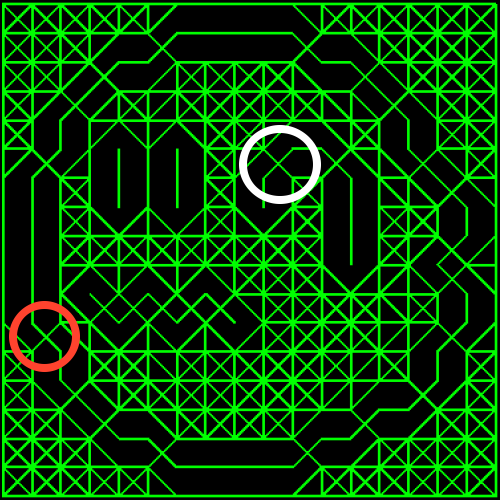
\includegraphics[width=\textwidth]{22}
        \caption{Initial graph}
        \label{fig:tiger}
    \end{subfigure}
    ~ %add desired spacing between images, e. g. ~, \quad, \qquad, \hfill etc. 
    %(or a blank line to force the subfigure onto a new line)
    \begin{subfigure}[b]{0.3\textwidth}
        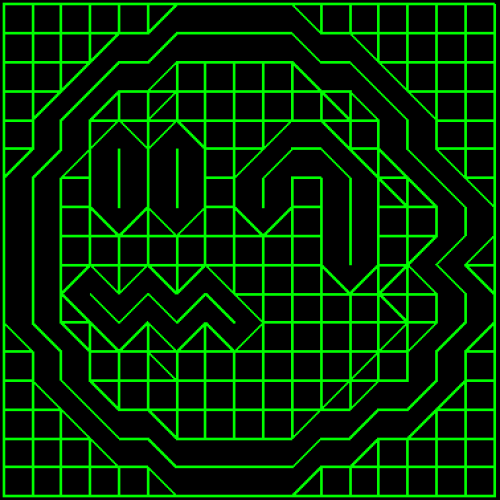
\includegraphics[width=\textwidth]{1}
        \caption{Planar graph}
        \label{fig:mouse}
    \end{subfigure}
    \caption{An example of creating planar connectivity graph. a: Original image, b: connectivity graph generated using YUV criteria, c: Planar graph received by applying three heuristics}\label{fig:animals}
\end{figure}

\subsection{Reshaping pixel cells}

The goal of this stage is to reshape the pixel cells that belong to the same feature so that they share an boundary instead of a vertex, which makes it to be clearly visible if two pixels are connected or not. Therefore, the shape of each pixel is decided by how it connects to its neighboring pixels.\begin{wrapfigure}{h}{0.15\textwidth}
    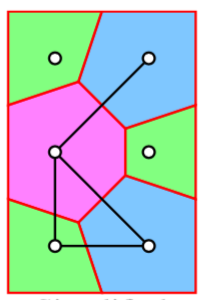
\includegraphics[width=0.15\textwidth]{diagram}
\end{wrapfigure}
If there is a connection between the pixel and its diagonal neighbor, a new edge lying between them with a pre-defined length is generated and then "provided" to each pixel. For each pixel, their shared vertex will be removed while two completely new vertexes are generated to replace the single old one. These two new vertexes actually locate inside their neighboring pixels.
By doing so, two diagonally connected pixels share two vertexes, which define an edge, and dramatically reduce the visual disconnection.
This procedure also effect other neighboring pixels since they also have to replace their old vertexes accordingly. The inset figure roughly demonstrates the procedure. The white circles mark the center of each pixel while the lines imply the connection. After applying the procedure, the pixel in the inset figure now have two new edges that it shares with its diagonal neighbors. 

\subsection{Fitting and optimizing b-spline curves}

The reshaped cell graph roughly defines the output image. The next step is to improve the smoothness of the edges which are now formed by consecutive line segments. This is done by replacing these edges by b-spline curves which are defined by the vertexes alongside the edge. 

\subsubsection{B-spline curves}

To generate a b-spline curve, we need to specify the knot vector and set of control points. Having knot vector and control points, a b-spline curve is defined as:

\[ C(u) = {\sum_{i=0}^n} N_{i,d}(u)P_i \]
Where $N_{i,d}(u)$ are the b-spline basis functions defined at each segment \textit{i} along the curve and degree \textit{u}, $P_i$ is the control point \textit{i-th}. The basis function $N_{i,d}(u)$ is generated by knot vector which is an increasing sequence of \textit{n+d} where \textit{n} is number of control points and \textit{d} is degree of b-spline.

In the scope of this work, there are two kinds of b-spline that are considered. The first one is clamped b-spline, as can be seen in Fig.\ref{fig:clamped}, which makes the b-spline passes by the first and last control points. This kind of b-spline can be acquired by repeating \textit{d+1} times the first and the last knot point.
The second one is closed b-spline, which is the curve defining a closed area (Fig.\ref{fig:closed}) and can be done by simply repeating \textit{d} first control points at the end of control point sequence. Utilizing these two kinds of b-spline helps generated b-splines to be connected to each other.

\begin{figure}
    \centering
    \begin{subfigure}[b]{0.4\textwidth}
        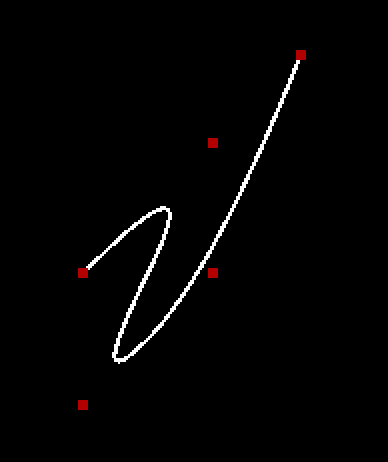
\includegraphics[width=\textwidth,height = \textwidth]{cl}
        \caption{Clamped curve}
        \label{fig:clamped}
    \end{subfigure}
    \begin{subfigure}[b]{0.4\textwidth}
        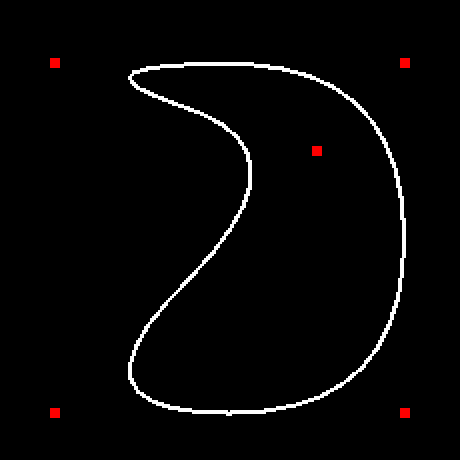
\includegraphics[width=\textwidth]{closed}
        \caption{Closed curve}
        \label{fig:closed}
    \end{subfigure}
    \caption{Example of clamped and closed curve}\label{fig:curve}
\end{figure}


\subsubsection{Extracting the Spline Curves}
At this point, only visible edges are considered. The visible edges are marked where significantly different color met, and is quantified by pre-defined thresholds. The valance of edge also counts visible edges only. The task now boils down to defining which sequence edges that should be replaced by a b-spline.
Fig.\ref{fig:vis} demonstrates the connections between the visible edges of reshaped pixel cells graph shown in Fig.\ref{fig:4}. One problem arises when three sequences end at a single node. Breaking down every things into separated curves is obviously not a good choice. In order to decide which sequences of edges should be connected to each other, all edges are classified into one among two kinds: either the contour edge or the shading edge based on two pixel cells defining them. An edge is defined as contour edge if the YUV distance of their two belonging pixels is larger than $100\over 255$. The types of edge are illustrated as colors in Fig.\ref{fig:vis} where tear edges are shading edges while the rest are contour edges. 

Having edges classified, the sequences of edges are defined such that each sequence is preferred to have same kind of edges. The search starts with contour edges at the node with high valance (marked with yellow for valence = 3 and violet for valence =4 in Fig.\ref{fig:vis}). Any sequences being found then is replaced by a b-spline taking the vertexes along the sequence as the control points.



\begin{figure}[h!]
\centering
    \begin{subfigure}[b]{0.3\textwidth}
        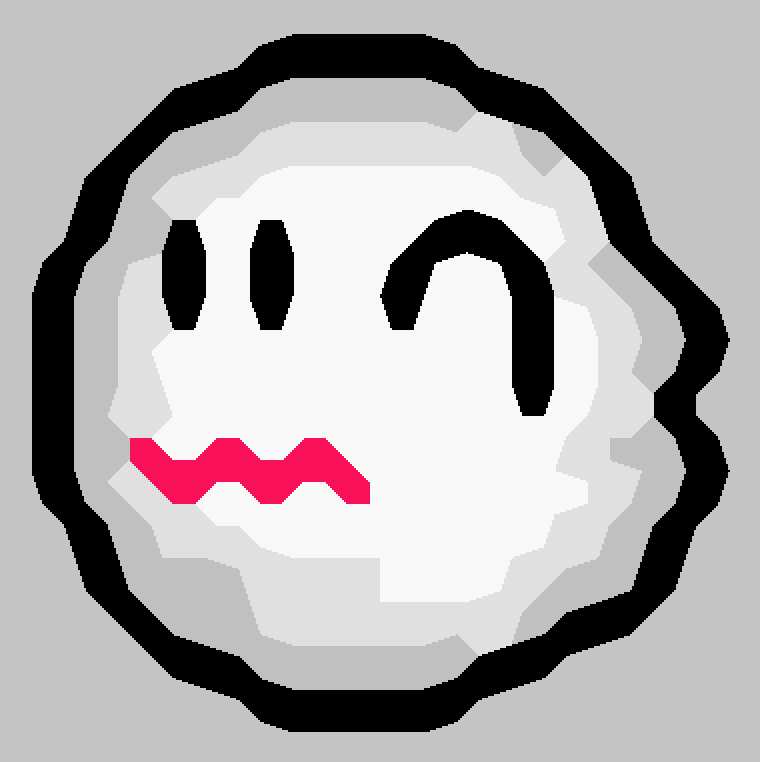
\includegraphics[width=0.8\textwidth]{4}
        \caption{ Reshaped cells graph }
        \label{fig:4}
    \end{subfigure}
    \begin{subfigure}[b]{0.3\textwidth}
        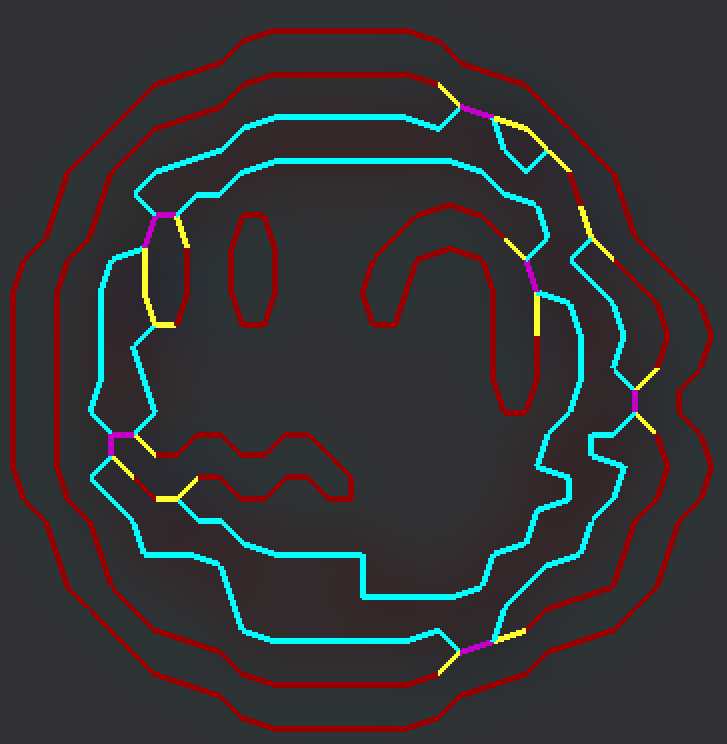
\includegraphics[width=0.8\textwidth]{vis}
        \caption{Visible edges}
        \label{fig:vis}
    \end{subfigure}
    \begin{subfigure}[b]{0.3\textwidth}
        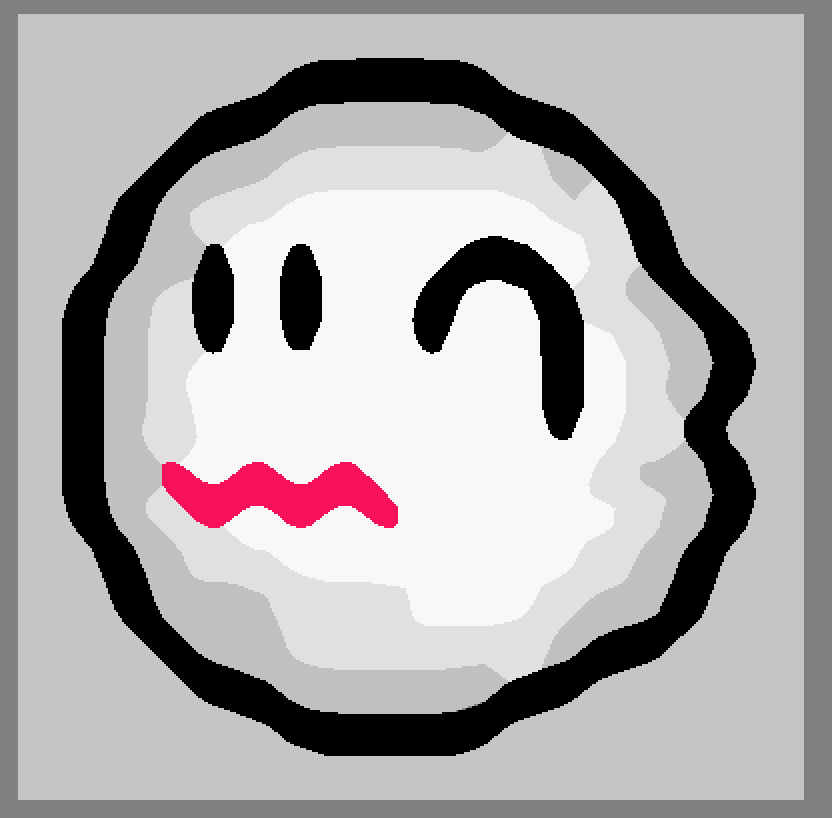
\includegraphics[width=0.8\textwidth]{5}
        \caption{Output}
        \label{fig:vis}
    \end{subfigure}
    \caption{ An example of the reshaped pixel cells graph, its visible edges, and the output after fitting the curves on the visible edges.}
    \label{vis}
\end{figure}

\subsubsection{Optimizing the curves}
This step is to enhance the smoothness of the curves by adjusting the position of their control points. The optimization therefore search in the space of control points' locations in order to minimize the energy terms defined as:
\[ Energy = \sum_i E_{smoothness}^{(i)} + E_{position}^{(i)} \]

Where the smoothness term is calculated by the absence of curvature which is formalized as:
\[ E_{smoothness}^{(i)} = \int_{s\in r(i)} |k (s)| \]
where $r(i)$ is the region of the curve that is under the effect of control point $p_i$ and $k(s)$ is the curvature at point $s$.
The integral can be approximated using the extended 2-point Newton-Cotes-Formula given as:
\[ \int_{x_1}^{x_n} f(x) dx = h({1\over2} f(x_1)+f(x_2)+f(x_3)...+ f(x_{n-2})+f(x_{n-1}) + {1\over 2} f(x_n)) \]
 where $x_i$ are uniformly sampled over the lower and upper bound of the integral and $h$ is distance between two consecutive points.

The second term of the energy is to ensure that the displacements possibly being made during the optimization are not too large. It penalizes the changes as follows:

\[ E_{position}^{(i)} = ||p_i - {p^"}_i ||^2 \]

where $p"$ are new points found during the optimization.

The optimization is then processed by a simple relaxation procedure: choosing randomly a point and optimizing the chosen points by trying random points in a small radius around its current location.
\Section{Results}
Fig. shows some representative results including variety of inputs from video games and other software. 

The limitation of the algorithm is illustrated in Fig.\ref{fail}. In the case of Fig.\ref{f3}, the algorithm fails to capture the main visible features since the colors encoded in the image vary significantly pixel by pixel. It is caused by intentionally arranging pixels with different colors side by side to acquire visual effect. This phenomenon happens quite often in modern pixel art where low-scale images are generated by interpolating from higher-resolution versions which containing many small details. Such kind of arrangement is against the main concept of this paper regarding the importance of every pixel. The third typical case shown in Fig.\ref{f1} and Fig.\ref{f2} clearly shows that the algorithm massively abuses the smoothness and turns out to be bad in some cases. 
\begin{figure}
  \centering
    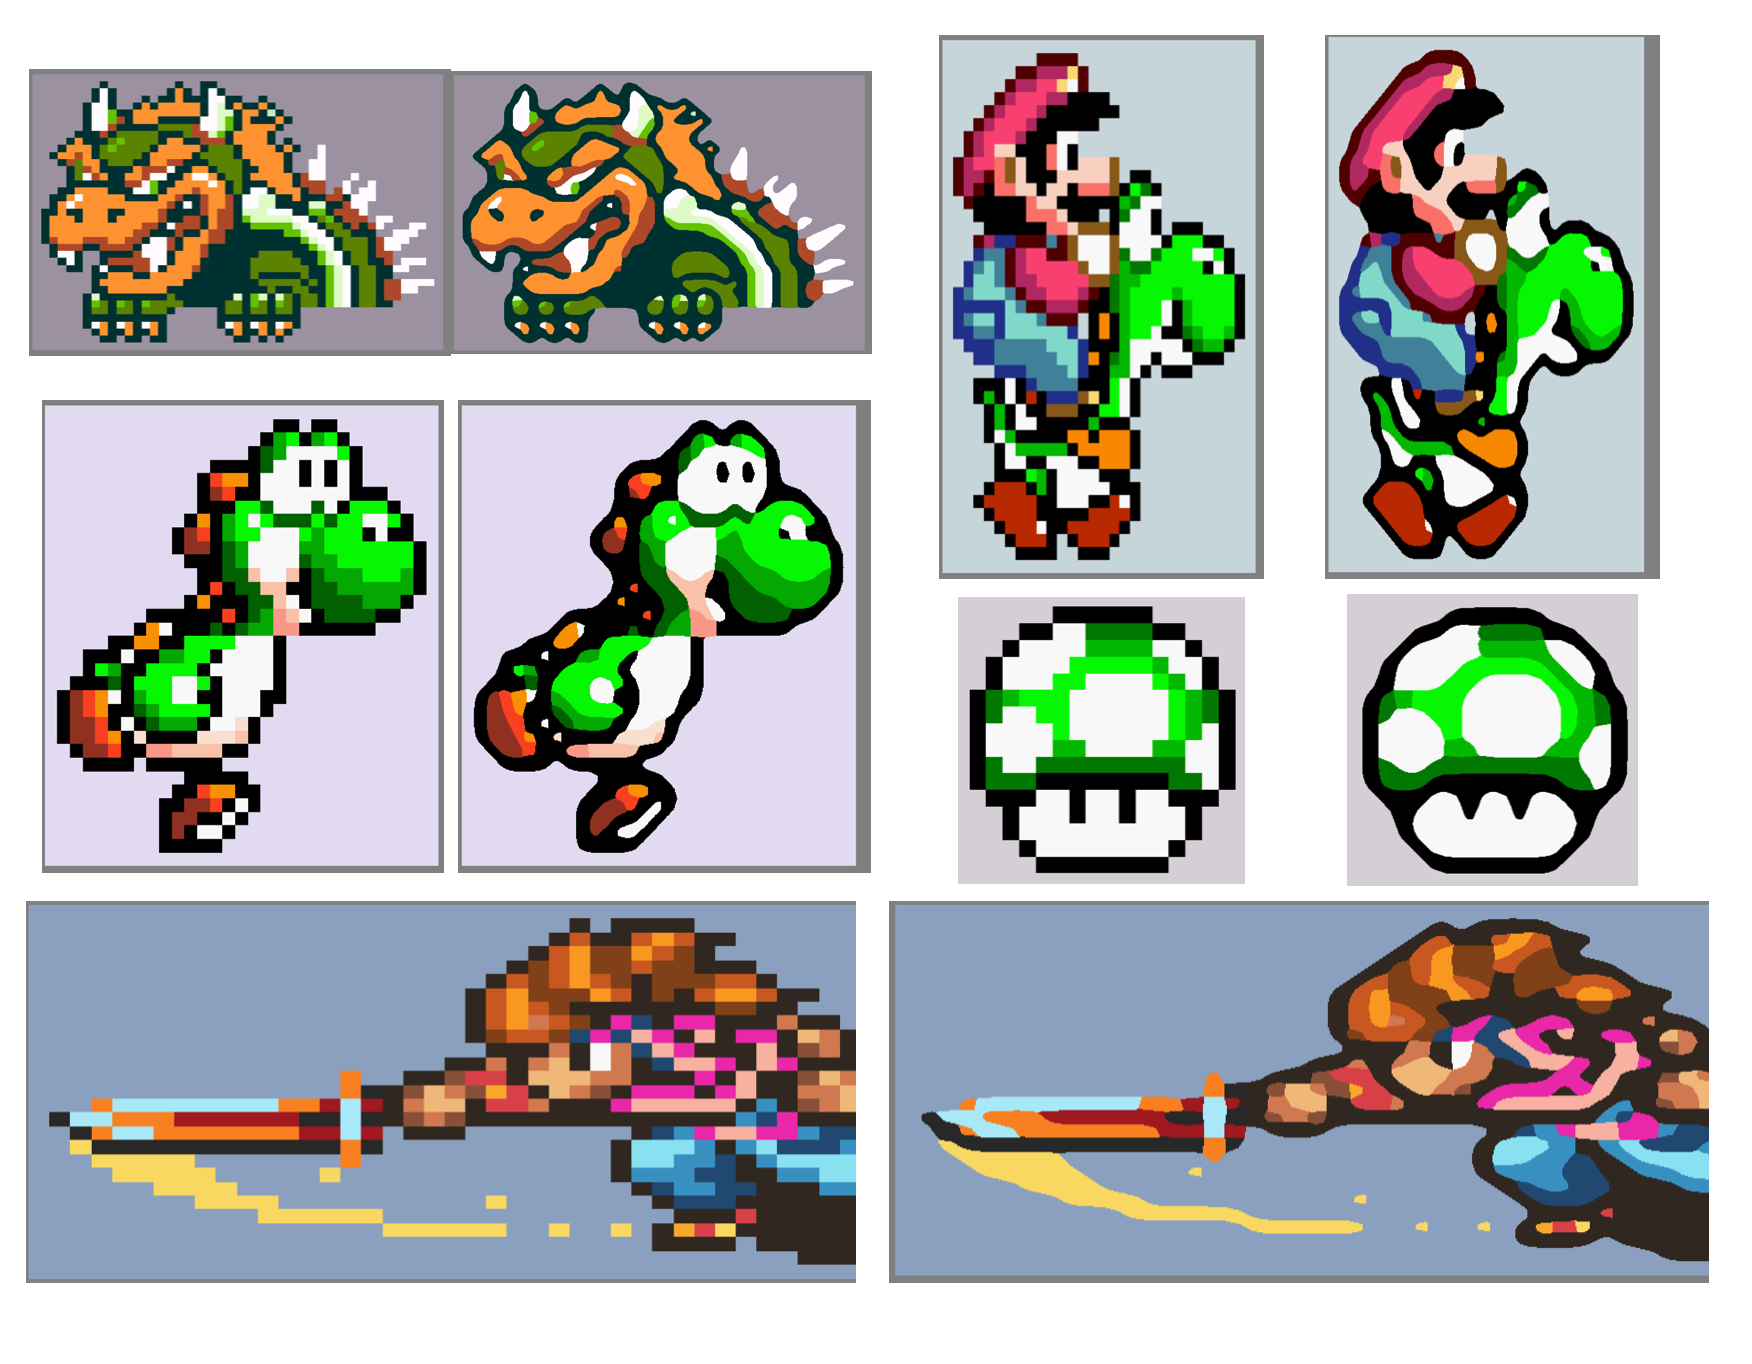
\includegraphics[width=\textwidth]{suc}
  \caption{Some example outputs of the algorithm.}
  \label{fig:suc}
\end{figure}

\begin{figure}[h!]
\centering
    \begin{subfigure}[b]{0.4\textwidth}
        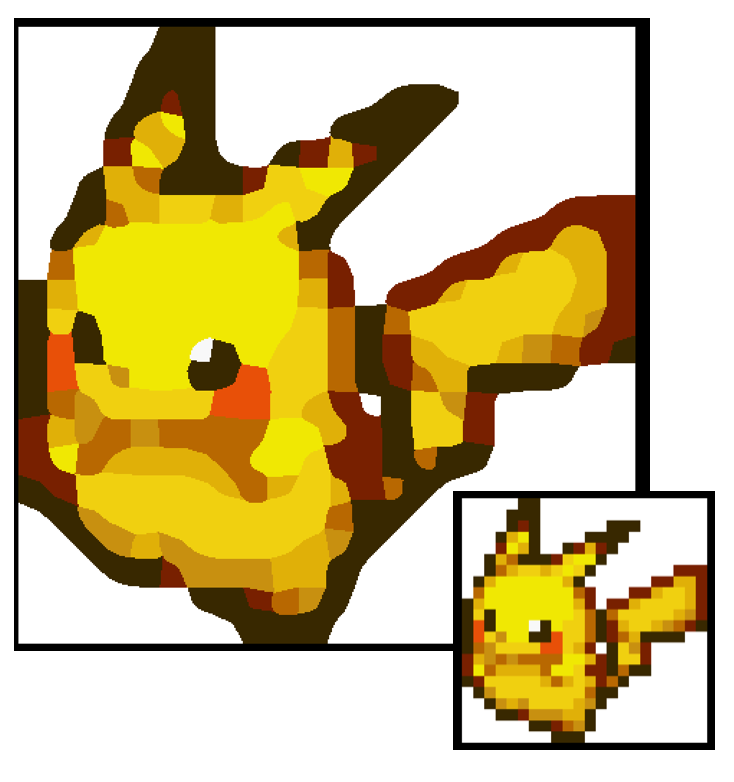
\includegraphics[width=1\textwidth]{f1}
        \caption{ Reshaped cells graph }
        \label{f1}
    \end{subfigure}
    \begin{subfigure}[b]{0.4\textwidth}
        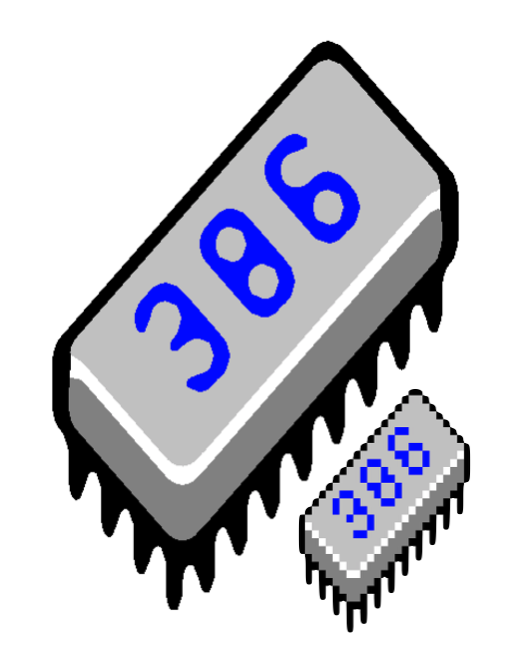
\includegraphics[width=\textwidth]{f2}
        \caption{Visible edges}
        \label{f2}
    \end{subfigure}
    \begin{subfigure}[b]{0.6\textwidth}
        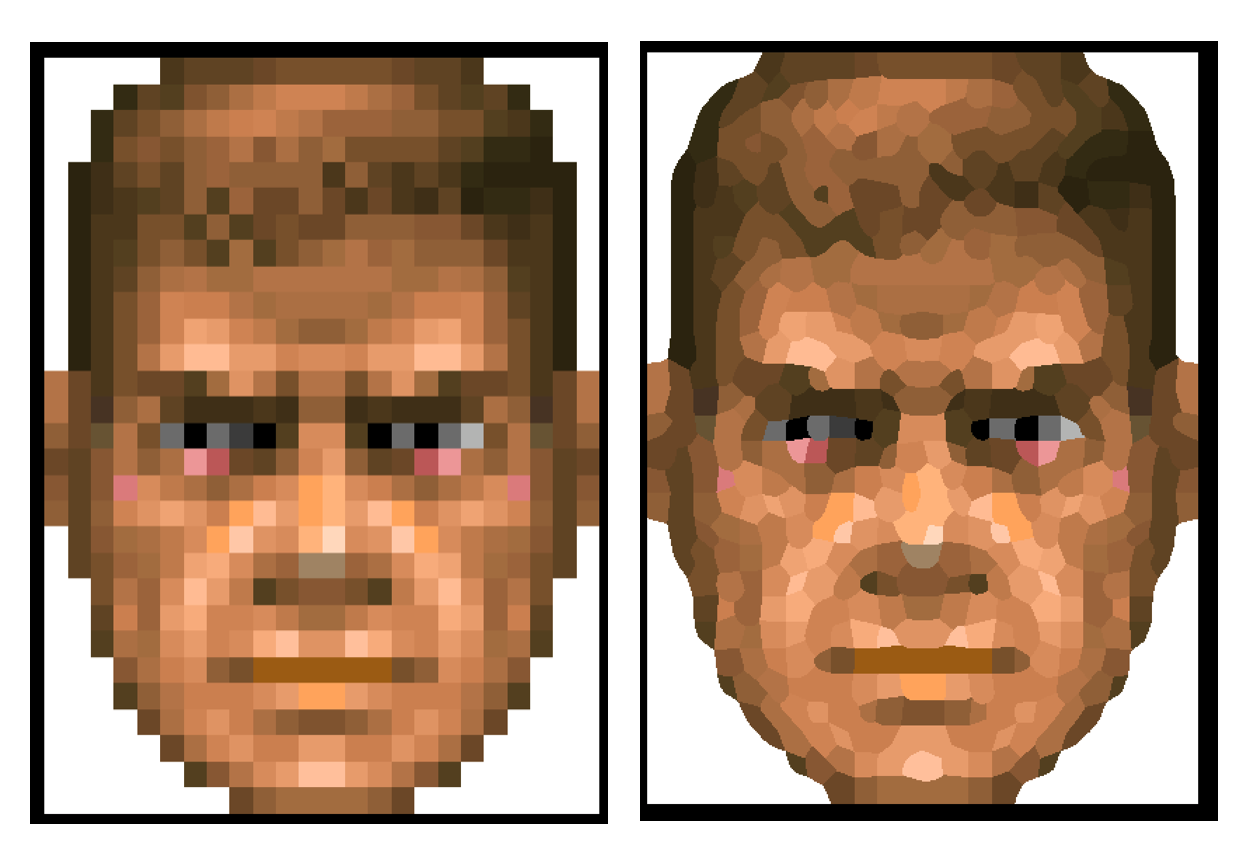
\includegraphics[width=\textwidth]{f3}
        \caption{Output}
        \label{f3}
    \end{subfigure}
    \caption{ Some examples that the algorithm fails to perform well.}
    \label{fail}
\end{figure}

\bibliographystyle{plain}
\bibliography{references}
\end{document}
